% !Mode:: "TeX:UTF-8"

\chapter{系统通用结构}
本申报系统是一个典型的管理信息系统[5](Management Information System)简称MIS。它是1961年在美国由J.D.Gdllagher首先提出的,并确定其以计算机为主体,信息处理为中心的综合性系统,由计算机技术、网络通讯技术、信息处理技术、管理科学和人组成的一个综合系统,能提供信息以支持一个组织机构的运行、管理和决策功能。

对于典型的MIS系统结构通过主要有三类[6]:\par
工作站、文件服务器结构的MIS系统。这种结构中,应用程序逻辑完全是在客户工作站上执行,一台或多台中央服务器提供了对于计算资源的访问途径。文件服务器只是提供文件访问服务,没有真正意义上的数据库引擎。这样所有程序逻辑均在客户端完成,容易造成客户端负担过重,随着基于客户机、服务器结构MIS的出现,使工作站、文件服务器结构的第一代MIS系统渐渐淡出主流MIS阵营。

C/S结构的MIS系统,这种结构借助于网络将应用资源和应用任务合理的分配到CLINET、SERVER两端。具体的,客户端主要功能是负责人机交互,管理用户接口、执行客户端应用程序,采集数据以及向服务器提交应用请求,而服务器则执行后台程序,主要承担数据库存储系统的共享管理、通讯管理、文件管理以及对客户机的请求提供服务。

B/S结构的MIS系统,这种结构与C/S模式相比,它简化了客户端的程序,通常在这种模式结构的系统中,客户端只需要一个浏览器就可以了。这种结构将许多工作交于WEB服务器来做,客户端只通过浏览器请求WEB服务,WEB服务器再根据不同请求返回信息,这其中还需请求数据库服务器以获取正确数据。因此,这种结构模式的MIS系统,而有瘦客户的称号,这是于C/S结构的胖客户相对而言的。

上述三种的系统结构,除第一种逐渐淡出之外,第二种与第三种都有大量的运用。通常如果要求系统的响应要求快,又是用于局域网内部或机关企事业单位内部的系统,可以采用C/S结构模式。但如果用户不在同一局域网内,而是分散在各个不再的地方或处于不同的单位,在这种情况下B/S结构模式通常比较适合。有时,在开发一个系统时,完成C/S结构模式、B/S结构模式两个版本的程序。也有些系统采用混合的模式,一部分功能模块采用C/S结构开发,而另一部分模块采用B/S结构开发。

考虑到质量申报系统的需求,该系统开发应用B/S结构开发。其主要功能如图~\ref{fig:func_mod}~所示。
\begin{figure}[htbp]
\centering
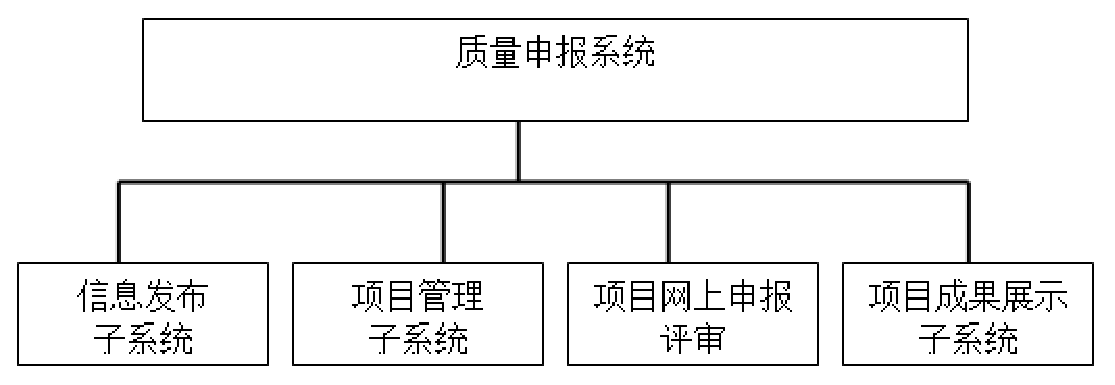
\includegraphics[width=14.6cm]{func_mod}
\caption{系统的主要功能模块}\label{fig:func_mod}
\vspace{\baselineskip}
\end{figure}
图中,各子系统的主要功能简介如下:

(1)	信息发布功能\par
主要是发布项目申报信息、项目指南、建设与改革动态等各类信息。

(2)	项目管理功能\par
主要进行项目分类、项目立项、项目建设过程管理、项目经费管理、项目结题验收管理、项目的统计分析和汇总管理。

(3)	项目的网上申报和网上评审功能\par
网上申报主要提供项目的网上申报功能,提供用户下载与填写申报书和上传申报书。网上评审主要结构专家对用户申报的项目进行评审。

(4)	项目成果展示交流功能\par
主要功能是展示项目的建设成果,并提供专家论坛、交流研讨等交互平台。为用户搭建一个沟通、交流、资源共享的平台。
